
\documentclass[10pt]{article}
\usepackage[a4paper, tmargin=0.75in, lmargin=0.80in, rmargin=0.80in, bmargin=1in]{geometry}
\usepackage{hyperref}
\usepackage{dsfont}
\usepackage{amsfonts}
\usepackage{ragged2e}
\usepackage{mathtools}
\usepackage{enumitem}   
\usepackage{MnSymbol}%
\usepackage{wasysym}%
\usepackage{relsize}%
\usepackage{xcolor}

\usepackage{amsmath}
\usepackage{upgreek}
\usepackage{mathrsfs}
\usepackage{blindtext}
\usepackage{listings}
\usepackage{xcolor}


%New colors defined below
\definecolor{codegreen}{rgb}{0,0.6,0}
\definecolor{codegray}{rgb}{0.5,0.5,0.5}
\definecolor{codepurple}{rgb}{0.58,0,0.82}
\definecolor{backcolour}{rgb}{0.95,0.95,0.92}

\lstset{
    literate={ĉ}{{\^c}}1
        {Ĉ}{{\^C}}1
}

%Code listing style named "mystyle"
\lstdefinestyle{mystyle}{
  backgroundcolor=\color{backcolour}, commentstyle=\color{codegreen},
  keywordstyle=\color{magenta},
  numberstyle=\tiny\color{codegray},
  stringstyle=\color{codepurple},
  basicstyle=\ttfamily\footnotesize,
  breakatwhitespace=false,         
  breaklines=true,                 
  captionpos=b,                    
  keepspaces=true,                 
  numbers=left,                    
  numbersep=5pt,                  
  showspaces=false,                
  showstringspaces=false,
  showtabs=false,                  
  tabsize=2
}

\lstset{style=mystyle}


\usepackage{natbib}
\usepackage{graphicx}
\pagestyle{empty}
\renewcommand\thesubsection{\Alph{subsection}}
\DeclareMathOperator*{\limop}{\lim}




%%%%%%%%%%%%%%%%%%%%%%%%%%%%%%%%%%%%%%%%%%%%%%%%%%
%%%%%%%%%%%%%%%%%%%%%%%%%%%%%%%%%%%%%%%%%%%%%%%%%%
%%%%%%%%%%%%%%%%%%%%%%%%%%%%%%%%%%%%%%%%%%%%%%%%%%
%%%%%%%%%%%%%%%%%%%%%%%%%%%%%%%%%%%%%%%%%%%%%%%%%%
% ENTER SOME IMPORTANT INFORMATION
%%%%%%%%%%%%%%%%%%%%%%%%%%%%%%%%%%%%%%%%%%%%%%%%%%
%%%%%%%%%%%%%%%%%%%%%%%%%%%%%%%%%%%%%%%%%%%%%%%%%%
%%%%%%%%%%%%%%%%%%%%%%%%%%%%%%%%%%%%%%%%%%%%%%%%%%
%%%%%%%%%%%%%%%%%%%%%%%%%%%%%%%%%%%%%%%%%%%%%%%%%%
\newcommand{\studentname}{Luis Alejandro Rubiano}
\newcommand{\studentnumber}{202013482}
\newcommand{\researchcentre}{la.rubiano@uniandes.edu.co}
\newcommand{\projecttitle}{Convex Optimization}
\newcommand{\supervisor}{Mauricio Junca}
\newcommand{\xRightarroww}[2][]{\ext@arrow 0359\Rightarrowfill@{#1}{#2}}

\newcommand\setItemnumber[1]{\setcounter{enum\romannumeral\@enumdepth}{\numexpr#1-1\relax}}

\newcommand\restr[2]{{% we make the whole thing an ordinary symbol
  \left.\kern-\nulldelimiterspace % automatically resize the bar with \right
  #1 % the function
  \littletaller % pretend it's a little taller at normal size
  \right|_{#2} % this is the delimiter
  }}

\newcommand{\littletaller}{\mathchoice{\vphantom{\big|}}{}{}{}}


%%%%%%%%%%%%%%%%%%%%%%%%%%%%%%%%%%%%%%%%%%%%%%%%%%
%%%%%%%%%%%%%%%%%%%%%%%%%%%%%%%%%%%%%%%%%%%%%%%%%%
%%%%%%%%%%%%%%%%%%%%%%%%%%%%%%%%%%%%%%%%%%%%%%%%%%
%%%%%%%%%%%%%%%%%%%%%%%%%%%%%%%%%%%%%%%%%%%%%%%%%%
%%%%%%%%%%%%%%%%%%%%%%%%%%%%%%%%%%%%%%%%%%%%%%%%%%
%%%%%%%%%%%%%%%%%%%%%%%%%%%%%%%%%%%%%%%%%%%%%%%%%%

\begin{document}

\begin{center}
{\Huge{Exam 1, Convex Optimization}} \\
\vspace{2mm}
{\Large{Departamento de Matemáticas, Universidad de los Andes}} \\
\vspace{1mm}
{\Large{Colombia}}
\end{center}

\vspace{5mm}
\hrule
\vspace{1mm}
\hrule

\vspace{3mm}
\begin{tabular}{ll} 
Student's name:           	        & {\studentname}   \\ 
Student's code: 	        & {\studentnumber} \\ 
Email address: 	        & {\researchcentre}  \\ 
Class: 	& {\projecttitle}  \\ 
Instructor: 	    & {\supervisor}  \\ 
\end{tabular}

\vspace{3mm}
\hrule
\vspace{1mm}
\hrule

\hfill \break %SPACE

\iffalse

\section{This exercise presents the concept of the convex conjugate of a function and its properties}

\begin{enumerate}[label=\alph*)]
  \item Let $C \subset \mathbb{R}^{n+1}$ convex and closed, such that it does not contain vertical lines, i.e. lines with direction $(0, \gamma), \gamma \neq 0$. Then, there is a nonvertical semispace, that contains it, that is, there are $a, \beta \neq 0$ and $\alpha$ such that $$ \langle a, x \rangle + \beta x_{n+1} \geq \alpha$$ for all $(x, x_{n+1}) \in C$.
\end{enumerate}

\paragraph{Proof:}


\blindtext

\begin{enumerate}[label=\alph*)]
\setcounter{enumi}{1}
\item Given $f: \mathbb{R}^n \rightarrow (- \infty, \infty]$, let the conjugate of $f$ be defined as: $$ f^*(y) = \sup_{x \in \mathbb{R}^n} \langle x, y \rangle - f(x) $$ 

\begin{enumerate}[label=\arabic*)]
  \item Show that $f^*$ is always convex, closed and $f^{**}(x) \leq f(x)$ for all $x \in \mathbb{R}^n$.
\end{enumerate}

\paragraph{Proof:}


\blindtext

\begin{enumerate}[label=\arabic*)]
  \setcounter{enumii}{1}
  \item Suppose that $f$ is closed and convex. Use a) to show that $f^{**} = f$.
\end{enumerate}

\paragraph{Proof:}


\blindtext


\begin{enumerate}[label=\arabic*)]
  \setcounter{enumii}{2}
  \item Suppose that $f$ is closed and convex. Show that the following properties hold:
  
\begin{enumerate}[label=(\roman*)]
  \item $\langle x,y \rangle = f(x) + f^*(y)$,
  \item $y \in \partial f(x)$,
  \item $x \in \partial f^*(y)$.
\end{enumerate}


\end{enumerate}


\paragraph{Proof:}

\blindtext

\begin{enumerate}[label=\arabic*)]
  \setcounter{enumii}{3}
  \item Find the conjugate of the function $f(x)= x \ln x$.
\end{enumerate}


\end{enumerate}

\section{Let $f: \mathbb{R}^n \rightarrow \mathbb{R}$ convex, and $c >0$.}

\begin{enumerate}[label=\alph*)]
  \item Let $g(x) = f(x) + \frac{1}{2c} \| x \|^2$, show that the level sets of $g$ are bounded.
\end{enumerate}

\paragraph{Proof:}

\blindtext

\begin{enumerate}[label=\alph*)]
  \setcounter{enumi}{1}
  \item Show that the function $\varphi(z) = \inf_{x} \{ f(x) + \frac{1}{2c} \| x- z\|^2 \}$ is convex and its minimum is attained at a unique point, for all $z \in \mathbb{R}^n$, denoted $x_z$.
\end{enumerate}

\paragraph{Proof:}

\blindtext

\begin{enumerate}[label=\alph*)]
  \setcounter{enumi}{2}
  \item Find $x_z$ when $f(x) = \chi_C(x)$, the characteristic function of a closed convex set $C$.
\end{enumerate}

\paragraph{Proof:}

\blindtext

\begin{enumerate}[label=\alph*)]
  \setcounter{enumi}{3}
  \item Show that $\cfrac{z-x_z}{c} \in \partial f(x_z)$.
\end{enumerate}

\paragraph{Proof:}

\blindtext

\begin{enumerate}[label=\alph*)]
  \setcounter{enumi}{4}
  \item Find $x_z$ when $f(x) = \|x\|_1$.
\end{enumerate}

\paragraph{Proof:}

\blindtext

\begin{enumerate}[label=\alph*)]
  \setcounter{enumi}{5}
  \item Show that $v \in \partial \phi(z)$ if and only if $(x_z, z)$ minimizes the function $(x,y) \mapsto f(x) + \frac{1}{2c} \| x - y \|^2 - \langle v, y \rangle$.
\end{enumerate}

\paragraph{Proof:}

\blindtext

\begin{enumerate}[label=\alph*)]
  \setcounter{enumi}{6}
  \item Use d) to show that $\phi$ is differentiable with $\nabla \phi(z) = \cfrac{z-x_z}{c} \in \nabla f(x_z)$ and conclude that $z$ minimizes $\varphi$ if and only if $z$ minimizes $f$.
\end{enumerate}

\paragraph{Proof:}

\blindtext

\fi

\setcounter{section}{2}

\section{In a multiclass classification problem with $s$ clases one has data of the form $(a,l) \in \mathbb{R}^n \times \{ 1, \ldots, s \}$, and one wants to find a linear classifier for each class, that is, 
one wants to find $x_l \in \mathbb{R}^n$ that minimizes the loss function $$ g(x_1, \ldots, x_s; a, l) = \max_{m \neq l} [ 1 + \langle a, x_m - x_l \rangle]_+$$
where $[t]_+ = \max \{ 0, t \}$. Note that given $(a,l)$, it is true that $g=0$ if and only if the 
classifiers of each class have a big margin, that is, for each $m \neq l$ one has that $$ \langle a, x_l \rangle \geq \langle a, x_m \rangle + 1.$$ Given a dataset $\{ (a_i, l_i) \}_{i=1}^N$ one wants to solve the problem $$\min \cfrac{1}{N} \sum_{i=1}^N g(x_1, \ldots, x_s; a_i, l_i) $$
  $$\text{ subject to } \|x_j\|_2 \leq r, j=1, \ldots, s.$$
Consider the database of handwritten digits (train.csv), in this case $n=784$ and $s=10$. From the more than $4000$ data for each digit, choose $N>5000$ and take $r=3$ to solve the problem with 
each of the following methods:}

Here the images were regularized to make them have norm $3$ (projection to the sphere of radius $3$). The subgradient was calculated in the following way:

\begin{itemize}
  \item Initialize $10$ arrays $\partial x_1, \ldots,\partial x_{10}$ with zeros.
  \item For each $(a, l)$ do:
  \begin{itemize}
    \item For $m$ from $1$ to $10$, $m \neq l$ do:
    \begin{itemize}
      \item Compute the value of $1+ \langle a_i, x_m - x_{l} \rangle$.
      \item If this value is greater than zero, save it
    \end{itemize}
    \item Find the maximum of the saved values, and its index $m$, if multiple values are the maximum, choose one randomly
    \item Augment the subgradient of $x_m$ by $a_i$ and decrease the subgradient of $x_l$ by $a_i$, this works because this will the derivative of one of the active restrictions, and thus it belongs to the subgradient of the objective function.
    \item Keep the other subgradients as they are. 
    \item This sum will be the subgradient of the objective function, as the subgradient of the sum of functions is the minkowski sum of the subgradients of each function.

  \end{itemize}
\end{itemize}

For the stochastic subgradient method, the batch size was $10$ and the stochastic subgradient was calculated as before but only for the $10$ data in the batch.\\

All the methods were given $5$ minutes to run. And $N$ was chosen to be $10000$ with $1000$ data for each digit.\\

\begin{enumerate}[label=\alph*)]
  \item Projected subgradient with step size $\alpha_k = \cfrac{\alpha}{\sqrt{k}}$ with $\alpha >0$. Say how you choose $\alpha$.
\end{enumerate}

\paragraph{Solution:}

In this case we used step size $\alpha = 10, 1, 0.1, 0.01$, here is the Python3 code for the projected subgradient method:

\begin{lstlisting}[language=Python]
alphas = [10, 1, 0.1, 0.01]

Fs_for_each = []

for alpha in alphas:
    Fs = []
    start = perf_counter()
    print(f'Alpha: {alpha}')
    k = 0
    X = array([rand(n) for _ in range(s)])
    for m in range(s):
        X[m] = r * X[m] / norm(X[m])

    while perf_counter() - start < 300: # 5 minutes
        a_k = alpha / sqrt(k+1)
        subgradient_at_X = subgradient(X, images, labels)
        for m in range(s):
            X[m] = X[m] - a_k * subgradient_at_X[m]
        # Project each X[m] to the unit ball
        for m in range(s):
            norm_X_m = norm(X[m])
            if norm_X_m <= r:
                continue
            else:
                X[m] = r * X[m] / norm_X_m
        if k % 50 == 0:
            print(f'Iteration {k} completed')
            print(f'Objective function value: {objective_function(X, images, labels)}')
        k += 1
        Fs.append(objective_function(X, images, labels))
    Fs_for_each.append(Fs)
\end{lstlisting}


\begin{enumerate}[label=\alph*)]
  \setcounter{enumi}{1}
  \item Projected subgradient with the $\alpha_k$ given by the Polyak step size. Say how you estimate $f^*$.
\end{enumerate}

\paragraph{Solution:}

In this case we used the Polyak step size, the $f^*$ was estimated by taking the value average for each pixel in the $10000$ images, and calculating the objetive function of that average. Here is the Python3 code for the projected subgradient method with Polyak step size:

\begin{lstlisting}[language=Python]
  print("\n"*3)
  f_star = 0.62988 # Optimal value of the objective function from testing
  Fs_Polyak = []
  start = perf_counter()
  k = 0
  X = array([rand(n) for _ in range(s)])
  for m in range(s):
      X[m] = r * X[m] / norm(X[m])
  
  while perf_counter() - start < 300: # 5 minutes
      a_k = (objective_function(X, images, labels) - f_star) / (norm(subgradient(X, images, labels))**2)
      subgradient_at_X = subgradient(X, images, labels)
  
      for m in range(s):
          X[m] = X[m] - a_k * subgradient_at_X[m]
      # Project each X[m] to the unit ball
      for m in range(s):
          norm_X_m = norm(X[m])
          if norm_X_m <= r:
              continue
          else:
              X[m] = r * X[m] / norm_X_m
      if k % 50 == 0:
          print(f'Iteration {k} completed')
          print(f'Objective function value: {objective_function(X, images, labels)}')
      k += 1
      Fs_Polyak.append(objective_function(X, images, labels))
\end{lstlisting}

\begin{enumerate}[label=\alph*)]
  \setcounter{enumi}{2}
  \item Stochastic subgradient with step size $\alpha_k = \cfrac{R}{L \sqrt{k}}$ and batch size $B=10$. Say how you choose $R$ and $L$.
\end{enumerate}

\paragraph{Solution:}

Here $R$ was chosen to be $10, 1, 0.1, 0.01$ and the Lipschitz constant was estimated by taking the norm of the stochastic subgradient of the objective function at each iteration. Here is the Python3 code for the stochastic subgradient method:

\begin{lstlisting}[language=Python]
  print("\n"*3)

  Rs = [10, 1, 0.1, 0.01]
  Fs_stochastic = []
  
  for R in Rs:
      Fs = []
      start = perf_counter()
      print(f'R: {R}')
      k = 0
      X = array([rand(n) for _ in range(s)])
      for m in range(s):
          X[m] = r * X[m] / norm(X[m])
  
      while perf_counter() - start < 300: # 5 minutes
          lipschitz_constants = []
          subgradient_at_X = stochastic_subgradient(X, images, labels)
          for m in range(s):
              a_k =  R / (sqrt(k+1) * norm(subgradient_at_X[m]))
              X[m] = X[m] - a_k * subgradient_at_X[m]
          # Project each X[m] to the unit ball
          for m in range(s):
              norm_X_m = norm(X[m])
              if norm_X_m <= r:
                  continue
              else:
                  X[m] = r * X[m] / norm_X_m
          if k % 50 == 0:
              print(f'Iteration {k} completed')
              print(f'Objective function value: {objective_function(X, images, labels)}')
          k += 1
          Fs.append(objective_function(X, images, labels))
      Fs_stochastic.append(Fs)
  
  # Save the results in csv
  df = DataFrame(Fs_for_each)
  df.to_csv('Fs_for_each.csv')
  
  df = DataFrame(Fs_Polyak)
  df.to_csv('Fs_Polyak.csv')
  
  df = DataFrame(Fs_stochastic)
  df.to_csv('Fs_stochastic.csv')  
\end{lstlisting}


\hfill \break %SPACE

To compare each of the methods do a graph of $f_k^*$ limiting the number of iterations of each method to the 
possibles in a time window that is the same for all. Detail all the calculations needed to implement the methods.

\begin{figure}[!tbp]
  \centering
  \begin{minipage}[b]{0.4\textwidth}
    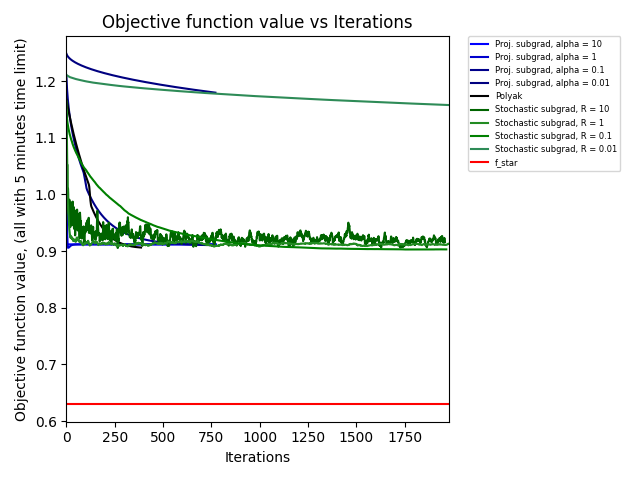
\includegraphics[width=\textwidth]{Objective_function_value_vs_Iterations.png}
    \caption{Objective function value vs Iterations}
    \label{fig:1}
  \end{minipage}
  \hfill
  \begin{minipage}[b]{0.4\textwidth}
    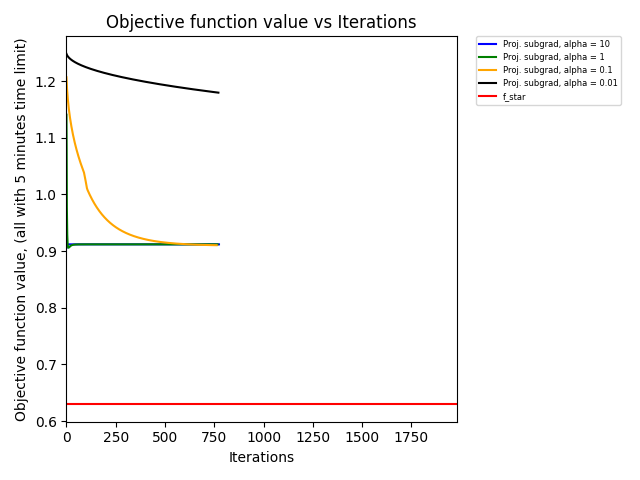
\includegraphics[width=\textwidth]{Projected_subgradient_vs_Iterations.png}
    \caption{Projected subgradient vs Iterations}
    \label{fig:2}
  \end{minipage}
\end{figure}

\begin{figure}[!tbp]
  \centering
  \begin{minipage}{0.45\textwidth}
    \centering
    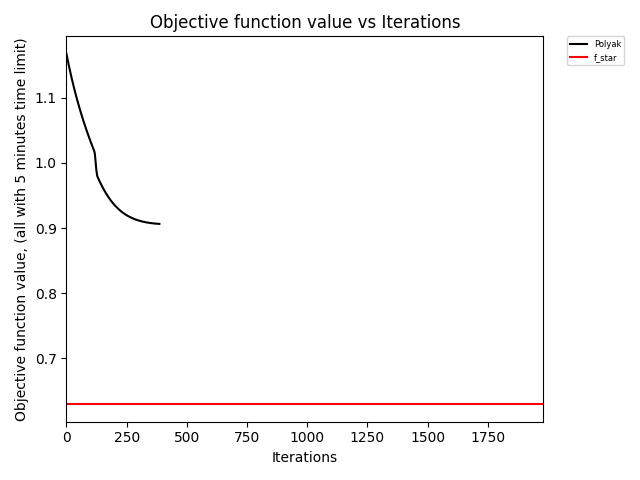
\includegraphics[width=\textwidth]{Polyak_vs_Iterations.png}
    \caption{Polyak vs Iterations}
    \label{fig:3}
  \end{minipage}
  \hfill
  \begin{minipage}{0.45\textwidth}
    \centering
    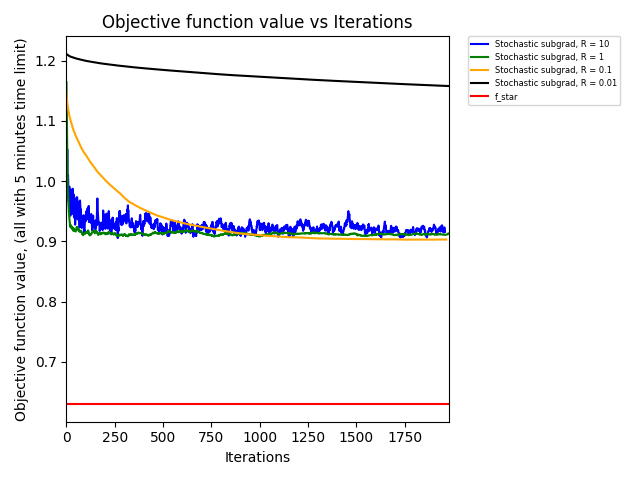
\includegraphics[width=\textwidth]{Stochastic_subgradient_vs_Iterations.png}
    \caption{Stochastic subgradient vs Iterations}
    \label{fig:4}
  \end{minipage}
\end{figure}

\end{document}